\graphicspath{{img/introduction/}}

% \begin{savequote}
% ``Trying to reinvent the wheel is a lot of work. It's okay to make some tweaks and enjoy the ride." 
%     \qauthor{Karen Lamb}
% \end{savequote}

\chapter{Introduction}
\label{chapter:introduction}

% \begin{synopsis}
% Background on DM and its current status
% \end{synopsis}
%%%%%%%%%%%%%%%%%%%%%%%%%%%%%%%%%%%%%
%%%%%%%%%%%%%%%%%%%%%%%%%%%%%%%%%%%%%
%%%%%%%%%%%%%%%%%%%%%%%%%%%%%%%%%%%%%

% Dark Matter is an enigma in modern physics. Despite the significant scientific % effort that has gone into trying to discern its nature, a definitive detection % proving its existence eludes us. Nevertheless, dark matter's influence % on our Universe is undeniable, with evidence supporting its existence arising on \fixMV{all} scales, large and small.

% \commMV{Cold collisionless fluid that explains many observations in astrophysics and cosmology. It's existence shouldn't be questioned, only its micro-physical constitution. }
%%%%%%%%%%%%%%%%%%%%%%%%%%%%%%%%%%%%%
%%%%%%%%%%%%%%%%%%%%%%%%%%%%%%%%%%%%% 
%%%%%%%%%%%%%%%%%%%%%%%%%%%%%%%%%%%%%
\section{Evidence for Dark Matter}
\label{ch1:sec:DM_evidence}
%%%%%%%%%%%%%%%%%%%%%%%%%%%%%%%%%%%%%
%%%%%%%%%%%%%%%%%%%%%%%%%%%%%%%%%%%%%
%%%%%%%%%%%%%%%%%%%%%%%%%%%%%%%%%%%%%

Today, the amount of evidence in support of dark matter's existence is overwhelming. This evidence comes from astrophysical and cosmological observations that are inconsistent with a universe composed entirely of visible matter. This section reviews this evidence. 

%%%%%%%%%%%%%%%%%%%%%%%%%%%%%%%%%%%%%
%%%%%%%%%%%%%%%%%%%%%%%%%%%%%%%%%%%%%
\subsection{Astrophysical Observations}
%%%%%%%%%%%%%%%%%%%%%%%%%%%%%%%%%%%%%
%%%%%%%%%%%%%%%%%%%%%%%%%%%%%%%%%%%%%

\subsubsection*{Galaxy Clusters}

Some of the first hints for the existence of dark matter came from observations of galaxy clusters. Perhaps the most famous analysis was performed by Fritz Zwicky~\cite{Zwicky:1937zza_MassesNebulaeClusters}, who was puzzled by the high rotational velocities of galaxies within the Coma Cluster. By applying the virial theorem, equating the cluster's kinetic and gravitational potential energies, he found that the cluster would need to contain a much more significant amount of \textit{dunkle materie} (dark matter) than visible matter to accommodate these high velocities.

\subsubsection*{Rotation Curves of Spiral Galaxies}

The anomalous rotational velocities observed in galaxy clusters can also be observed at the galactic scale. The rotation curves of spiral galaxies, which relate the rotational velocities of stars to their distance from the galactic centre, were observed to be flat at large distances. From the observed distribution of visible matter, Newtonian mechanics predicts that the orbital velocity of a star a distance $r$ from the galactic centre, $v_\star(r)$, is related to the mass contained within a radius $r$, $M(r)$, through
\begin{equation}
    v_\star(r) = \sqrt{\frac{G M(r)}{r}},
\end{equation}
indicating that the velocity should fall off as $1/\sqrt{r}$ at the outer regions of the galaxy where $M(r)$ is constant. Instead, observations of many spiral galaxies indicate that this velocity remains constant out to the galaxy's edge. 

A simple way to produce such a rotation curve is to introduce a spherically symmetric distribution of dark matter surrounding the galaxy,
\begin{equation}
    \rho_{\mathrm{DM}}(r) = \frac{v_0^2}{4 \pi G r^2},
\end{equation}
which results in a constant rotational velocity of $v_0$ out to the galaxy edge. Detailed simulations of structure formation in a Cold Dark Matter (CDM) Universe indicate that the true distribution is better represented by distribution functions such as the Navarro-Frenk-White (NFW) profile~\cite{Navarro:1995iw_StructureColdDark, Navarro:1996gj_UniversalDensityProfile} or Einasto~\cite{Einasto_jan_ConstructionCompositeModel} profiles, which are commonly used in the literature.
% \begin{equation}
%     \rho_{\mathrm{DM}}(r) = \frac{\rho_0}{\left( \frac{r}{r_\mathrm{s}}\right)\left( 1 + \frac{r}{r_\mathrm{s}}\right)^2},
% \end{equation}
% respectively, where $\rho_0$ and $r_\mathrm{s}$ are free parameters that must be fit to each halo. 
% More detailed simulations show that the true profile deviates slightly from an NFW, instead being more appropriately modeled by an Einasto profile. However, both profiles are observationally indistinguishable.

An example rotation curve for galaxy NGC 6503 is presented in Fig.~\ref{ch1:fig:gal_rotn_curve}, with the contributions from each of the matter components to the rotational velocity shown~\cite{Freese:2008cz_may_ReviewObservationalEvidence, Lelli:2016zqa_SPARCMassModels}. As can be seen, the visible matter constituting disk and gas components does not explain the observed rotational velocity. 

\begin{figure}[t!]
    \centering
    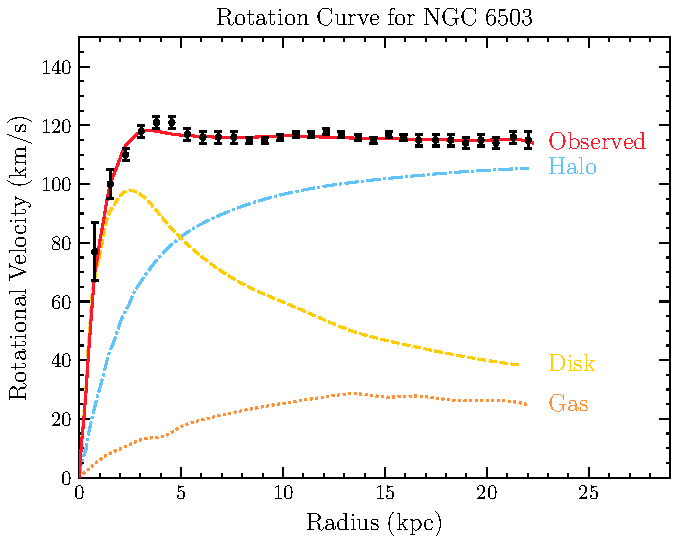
\includegraphics{gal_rotn_N6503}
    \caption[Galaxy rotation curve for NGC 6503.]{Galaxy rotation curve for NGC 6503, showing the contributions to the total velocity (red) from the DM halo (blue), disk (yellow), and gas components. Data used in making this plot was obtained from~\cite{Freese:2008cz_may_ReviewObservationalEvidence, Lelli:2016zqa_SPARCMassModels}.}
    \label{ch1:fig:gal_rotn_curve}
\end{figure}

\subsubsection*{Gravitational Lensing}

As described by General Relativity, the curvature of space-time around massive entities causes light to travel along curved paths. 
As such, the mass of astrophysical structures can be deduced from the extent to which they distort the images of objects in the background. The extent of the distortions depends on how massive the foreground object is, ranging from the shearing of the background image (weak lensing), to multiple copies of the background object appearing (strong lensing)~\cite{Schneider_Gravitationallensingstrong}.  The disparity between the mass obtained from gravitational lensing and the mass of visible matter in the system is further evidence of dark matter's existence~\cite{SDSS:2005sxd_FourthDataRelease, Mandelbaum:2005nx_Galaxyhalomasses}. 

\subsubsection*{The Bullet Cluster}
Galaxy cluster 1E 0657-56, commonly referred to as the ``bullet cluster'', was formed by the collision of two separate galaxy clusters. 
The baryonic matter in these clusters is mostly composed of a strongly interacting gas and, as expected, produced a significant amount of X-rays during the collision. These X-rays were imaged by the Chandra X-Ray telescope~\cite{Clowe:2003tk_Weaklensingmass}, providing information on the resulting distribution of the visible matter. This is shown by the red regions of Fig.~\ref{ch1:fig:bullet_cluster}, where it can be seen how the visible matter has been smeared due to the collision. 
However, when the gravitational potential was mapped using gravitational lensing, it was clear that the majority of the mass was displaced relative to the visible matter. This mass is attributed to the dark matter components of the original clusters. As indicated by the purple regions in Fig.~\ref{ch1:fig:bullet_cluster}, the dark matter halos seem to have passed through each other mostly unperturbed. This tells us that not only is the majority of the mass comprised of dark matter, but that the dark matter has extremely weak interactions with both the visible matter and itself. 

\begin{figure}[t!bp]
    \centering
    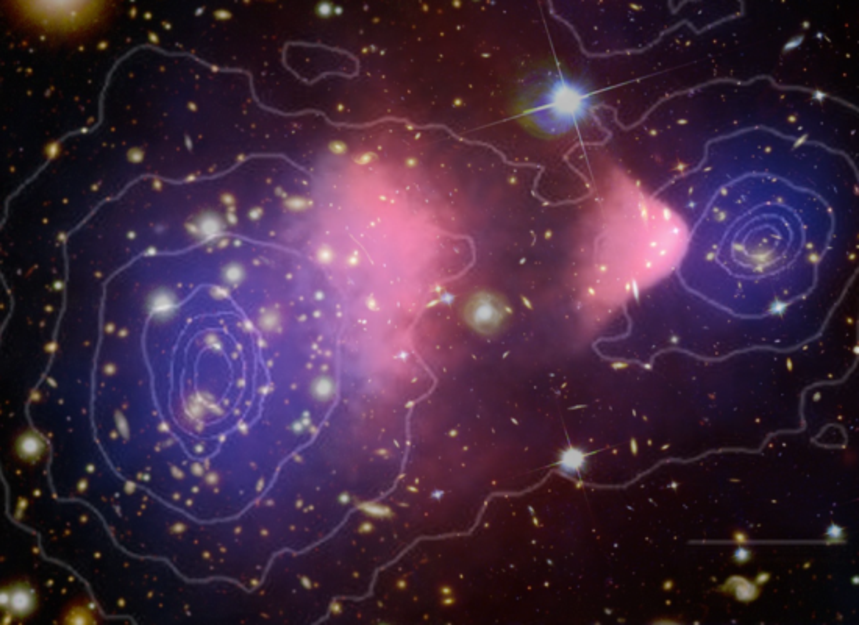
\includegraphics[width = 0.75\textwidth]{bullet_cluster}
    \caption[Image of the Bullet Cluster with contours of the gravitational potential superposed.]{Image of the Bullet Cluster with contours of the gravitational potential superposed. The red regions indicate the baryonic matter after the collision, while the purple regions are the expected DM components deduced from gravitational lensing. \cite{Clowe:2003tk_Weaklensingmass,Randall:2008ppe_ConstraintsSelfInteractionCrossSection}}
    \label{ch1:fig:bullet_cluster}
\end{figure}

%%%%%%%%%%%%%%%%%%%%%%%%%%%%%%%%%%%%%
%%%%%%%%%%%%%%%%%%%%%%%%%%%%%%%%%%%%%
\subsection{Cosmological Evidence}
\label{ch1:subsec:cosmo_evidence}
%%%%%%%%%%%%%%%%%%%%%%%%%%%%%%%%%%%%%
%%%%%%%%%%%%%%%%%%%%%%%%%%%%%%%%%%%%%
 
The current best cosmological model is the $\Lambda$-Cold Dark Matter model ($\Lambda$CDM), in which $\Lambda$ refers to the cosmological constant associated with dark energy, and as the name suggests, cold (i.e. non-relativistic) dark matter plays a prominent role. The key components of this model are the aforementioned dark energy and dark matter, along with baryonic matter, and it assumes that gravity is described by Einstein's General Relativity. The total energy density of the universe, $\rho_\mathrm{Univ.}$, can be broken down into three components based on how their density redshifts with the expansion of the Universe. In the $\Lambda$CDM model, these components are matter, radiation, and the vacuum energy $\Lambda$. The cosmological abundances of each component, ($\Omega_\mathrm{m}$, $\Omega_\mathrm{r}$, $\Omega_\Lambda$ respectively), are expressed as a fraction of the critical density, $\rho_\mathrm{crit}$,     
\begin{align}
    \rho_\mathrm{crit}   & = \frac{H^2}{8 \pi G_N},\\
    \Omega_i & = \frac{\rho_i}{\rho_\mathrm{crit}},
\end{align}
where $H$ is the Hubble parameter, such that the total energy density of the Universe satisfies
\begin{equation}
    \Omega_\mathrm{m} + \Omega_\mathrm{r} + \Omega_\Lambda = \frac{\rho_\mathrm{Univ.}}{\rho_\mathrm{crit}} \equiv \Omega_\mathrm{tot}.
\end{equation}
The ratio $\rho_\mathrm{Univ.}/\rho_\mathrm{crit}$ determines the curvature of the universe, with values greater than 1 corresponding to a closed universe, less than 1 to an open universe, and equal to 1 to a spatially flat universe. Current observations are consistent with a spatially flat universe, and so we have $\sum_i \Omega_i = 1$.


The $\Lambda$CDM model has seen huge success as it provides explanations for the observed power spectrum of the Cosmic Microwave Background (CMB), the large-scale structure of the Universe, the abundances of light elements (hydrogen, deuterium, helium, and lithium), and the accelerated expansion rate of the Universe. These observations constrain the parameters of the model and hence provide a complimentary probe of the properties of dark matter to the astronomical observations discussed above.

\subsubsection*{The Cosmic Microwave Background}
One of the strongest probes of cosmological models is the Cosmic Microwave Background (CMB), relic photons from the epoch of last scattering. This occurred after recombination, at a temperature of around $\sim 3000 \K$, once the photons had decoupled from the baryonic matter and could freely propagate through the universe. The photons observed today have been redshifted by the expansion of the Universe and are well described by a blackbody spectrum with a temperature of $T_\mathrm{CMB} = 2.73\pm 0.0006\K$. Observations of the CMB temperature reveal that it is not exactly isotropic, with anisotropies at the level of $\delta T_\mathrm{CMB}/T_\mathrm{CMB}\sim 10^{-5} - 10^{-6} $ seen on a range of angular scales in the sky. These anisotropies were seeded by the primordial density perturbations that arise during inflation. These perturbations evolve due to the acoustic oscillations of the photon-baryon plasma driven by the interplay between the pressure from the photons and the gravitational attraction of the matter. The oscillations cease once the photons decouple, freezing in their temporal phases that are observed as peaks in the angular power spectrum of the temperature anisotropies. 

Measurements of the CMB power spectrum provide information on many of the cosmological parameters, including $\Omega_\mathrm{tot}$, $\Omega_\mathrm{b}$ and $\Omega_\mathrm{DM}$.
% The locations of the acoustic peaks depend on the spatial geometry of the Universe and hence constrains $\Omega_\mathrm{tot}$. The total matter density, $\Omega_\mathrm{m}$, affects how the CMB spectrum is gravitationally lensed.  The relative amplitudes of the peaks probe the baryon-to-photon ratio and hence the baryon density, $\Omega_\mathrm{b}$. Finally, the density of dark matter, $\Omega_\mathrm{DM}$, is obtained by fitting the cosmological parameters to the exact shape of the spectrum~\cite{Freese:2008cz_may_ReviewObservationalEvidence, Planck:2018vyg_sep_Planck2018results}. 
The Planck collaboration most recently performed a precise measurement of the CMB power spectrum in 2018, obtaining best-fit parameters~\cite{Planck:2018vyg_sep_Planck2018results,Planck:2019nip_sep_Planck2018results}
\begin{equation}
     \Omega_\mathrm{m} = 0.311 \pm 0.006,\quad \Omega_\Lambda = 0.689 \pm 0.006,
\end{equation}
for the matter and dark energy densities. They obtained a total energy density of $\Omega_\mathrm{tot} = 1.011 \pm 0.006$ at $68\%$ confidence level, providing strong evidence for a spatially flat Universe. 
The breakdown of the matter density into the dark and baryonic components is determined by combining the CMB results with constraints from Big Bang Nucleosynthesis (BBN)\footnote{BBN is the process in which the light elements (D, $\ce{^3 He}$, $\ce{^4 He}$, and $\ce{^7 Li}$) were produced in the early universe.} giving
\begin{equation}
    \Omega_\mathrm{DM}h^2 = 0.1193 \pm 0.0009,\quad \Omega_\mathrm{b}h^2 = 0.02242 \pm 0.00014,
\end{equation}
where $h$ is the dimensionless Hubble constant such that the Hubble parameter today is $H_0 = 100\, h\km\s^{-1}\;\mathrm{Mpc}$. 


% The result for the baryon density is consistent with the value obtained from Big Bang Nucleosynthesis (BBN), the process in which light elements are formed in the early universe. BBN gives a baryon density of $\Omega_\mathrm{b} = 0.0220 \pm 0.0004$, in good agreement with the CMB result.


\subsubsection*{Large Scale Structure}
% After recombination, the pressure on the baryonic matter from photons began to decrease, eventually allowing the small density perturbations to grow. This led to the growth of the large-scale structure we observe today~\cite{Springel:2006vs_LargescalestructureUniverse}. 
The large-scale structure that we observe in our universe would not be possible without the presence of dark matter in the early universe.
N-body simulations of the Universe's evolution require a cold dark matter component for this structure to form. While a small component of the dark matter can be warm, hot dark matter would wash out small-scale structures~\cite{Springel:2005nw_Simulatingjointevolution}.  

%%%%%%%%%%%%%%%%%%%%%%%%%%%%%%%%%%%%%
%%%%%%%%%%%%%%%%%%%%%%%%%%%%%%%%%%%%%
%%%%%%%%%%%%%%%%%%%%%%%%%%%%%%%%%%%%%
\section{Potential Models of Dark Matter}
\label{ch1:sec:DM_models}
%%%%%%%%%%%%%%%%%%%%%%%%%%%%%%%%%%%%%
%%%%%%%%%%%%%%%%%%%%%%%%%%%%%%%%%%%%%
%%%%%%%%%%%%%%%%%%%%%%%%%%%%%%%%%%%%%

Given that all baryonic matter is composed of fundamental particles described by the Standard Model (SM) of particle physics, it is reasonable to assume that dark matter will also have a particle nature. Given the few details we know about dark matter, there exists an enormous library of models that predict a viable dark matter candidate.
These models may be as simple as adding a single new field to the SM, or there may be a more extensive hidden sector with a complicated symmetry structure. Additionally, there are models in which dark matter is not a fundamental particle, such as primordial black holes (PBHs) that formed in the early universe. There are several generic properties that a good dark matter candidate must satisfy, namely:

\begin{itemize}
    \item \textbf{Stable on Cosmological Timescales:} Dark matter must either be stable or have a lifetime significantly longer than the age of the Universe to be present in its current abundance. 
    
    \item \textbf{Neutral or milli-charged under Electromagnetism:} Dark matter, as its name suggests, does not significantly interact with light. Requiring that dark matter be completely decoupled from the Standard Model plasma by the time of recombination yields an upper bound on the electric charge of dark matter~\cite{McDermott:2010pa_TurningLightsHow} 
    \begin{equation}
        q_\mathrm{DM}/e < \begin{cases}
            3.5\times10^{-7} \left( \frac{m_\mathrm{DM}}{1\GeV}\right)^{0.58},\quad m_\mathrm{DM} > 1\GeV\\
            4.0\times 10^{-7}\left( \frac{m_\mathrm{DM}}{1\GeV}\right)^{0.35},\quad m_\mathrm{DM} <1\GeV
        \end{cases}
    \end{equation}
    
    \item \textbf{Small Self-Interactions:} The standard $\Lambda$CDM cosmology assumes that the dark matter is collisionless. However, small dark matter self-interactions can help resolve existing small-scale structure issues~\cite{Tulin:2017ara_feb_DarkMatterSelfinteractions, Spergel:1999mh_Observationalevidenceselfinteracting}. Current limits on the self-interaction cross-section are $\sigma_{\mathrm{DM-DM}}/m_\mathrm{DM} < 0.48\cm^2/\mathrm{g}$ which come from merging galaxy clusters~\cite{Randall:2008ppe_ConstraintsSelfInteractionCrossSection} and the ellipticity of galaxies obtained from X-ray observations~\cite{Buote:2002wd_ChandraEvidenceFlattened}.

    \item \textbf{Cold:} Dark matter is required to be non-relativistic at the time of structure formation. At most, a small component of the dark matter can be warm (semi-relativistic).
\end{itemize}
A selection of the more prominent dark matter candidates is shown in Fig.~\ref{ch1:fig:DM_models_landscape}. The key features of a few of these models are discussed below.

%%%%%%%%%%%%%%%%%%%%%%%%%%%%%%%%%%%%%%%%%
\begin{figure}[t!]
    \centering
    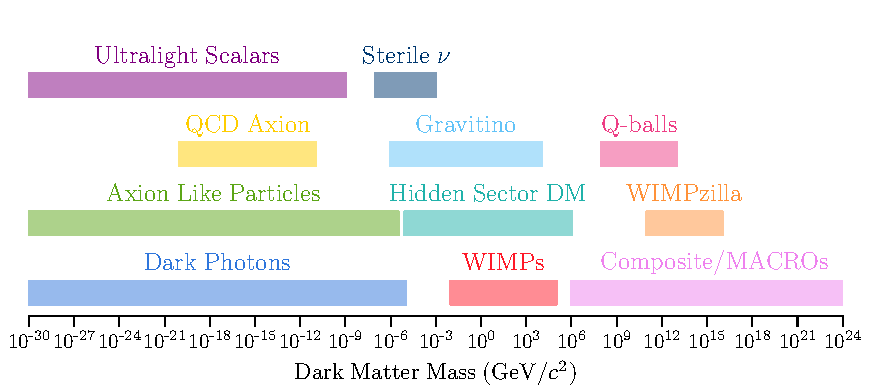
\includegraphics{DM_model_landscape}
    \caption[Mass ranges for various models of dark matter.]{Mass ranges for various models of dark matter. Details can be found in Chapter 26 of the PDG~\cite{ParticleDataGroup:2022pth_aug_ReviewParticlePhysics}.}
    \label{ch1:fig:DM_models_landscape}
\end{figure}
%%%%%%%%%%%%%%%%%%%%%%%%%%%%%%%%%%%%%%%%%

\subsubsection*{WIMPs}
Weakly Interacting Massive Particles (WIMPs) are a class of dark matter candidates that generically have masses and interaction strengths around the weak scale. Many extensions of the SM naturally predict the existence of such a particle, with famous examples being the lightest supersymmetric particle in supersymmetric theories~\cite{Goldberg:1983nd_ConstraintPhotinoMass}, or the lightest stable Kaluza-Klein mode in theories with extra dimensions~\cite{Kolb:1983fm_DimensionalReductionEarly}. 

In recent times, the term ``WIMP dark matter" is used almost synonymously to mean thermal relic, referring to a species whose relic abundance is produced thermally in the early universe through the freeze-out mechanism~\cite{Jungman:1995df_Supersymmetricdarkmatter}.
In this paradigm, the WIMP is initially in thermal equilibrium with the Standard Model bath. This equilibrium is maintained as long as the interaction rates of the WIMP with the bath, denoted $\Gamma$, remain faster than the Hubble expansion of the universe, $H$. As the universe continues to expand, the temperature of the bath drops, slowing down the interaction rates. Eventually, the expansion rate overtakes the interaction rates, $\Gamma/H\lesssim 1$, and the interactions ``freeze out'' causing the WIMP to fall out of equilibrium with the bath. At this point, the WIMPs can no longer efficiently annihilate, and their abundance gets ``frozen-in'' to the value it had at freeze-out, leading to the abundance observed today. 


A cold thermal relic, such as dark matter, will freeze out after it has become non-relativistic. In this scenario, the interaction rates become Boltzmann suppressed\footnote{The number density of a non-relativistic species of mass $m$ that is in thermal equilibrium with the bath will follow $n \propto \left(m T_\mathrm{bath}\right)^{3/2} \exp\left(-m /T_\mathrm{bath}\right)$. Once the temperature falls below the mass of the species, the number density becomes exponentially suppressed. This is what is known as ``Boltzmann suppression''.}, and the species rapidly freezes out. The relic density is therefore sensitive to the annihilation cross-section of the species, $\langle \sigma_\mathrm{ann} v\rangle$. More efficient annihilations correspond to larger cross-sections, resulting in the species remaining in equilibrium for longer times. This allows the number density to continue following the exponentially decreasing Boltzmann distribution and yield a smaller relic abundance. The evolution of the abundance of a Majorana fermion WIMP of mass $m_\mathrm{WIMP} = 100\GeV$ is shown in Fig.~\ref{ch1:fig:WIMP_freezeout} for three values of the annihilation cross-section. A simple expression  relating the annihilation cross-section and the abundance that is correct to $\sim5\%$ can be obtained~\cite{Steigman:2012nb_PreciseRelicWIMP} 
\begin{align}
    \Omega_{\mathrm{DM}}h^2 & = \frac{10^{-27}\cm^3\s^{-1}}{\sigmav} \frac{x_*}{g_*^{1/2}}\\
     &\sim 0.12 \; \left(\frac{2.2\times 10^{-26}\cm^3 \s^{-1}}{\langle \sigma v\rangle}\right),\quad m_\chi\gtrsim 10\GeV,
\end{align}
where $x_* = m_\mathrm{WIMP}/T_*$ is evaluated at an intermediate temperature between equilibrium and freeze-out, with $g_*$ the effective number of relativistic degrees of freedom present at this time. 

\begin{figure}[t!]
    \centering
    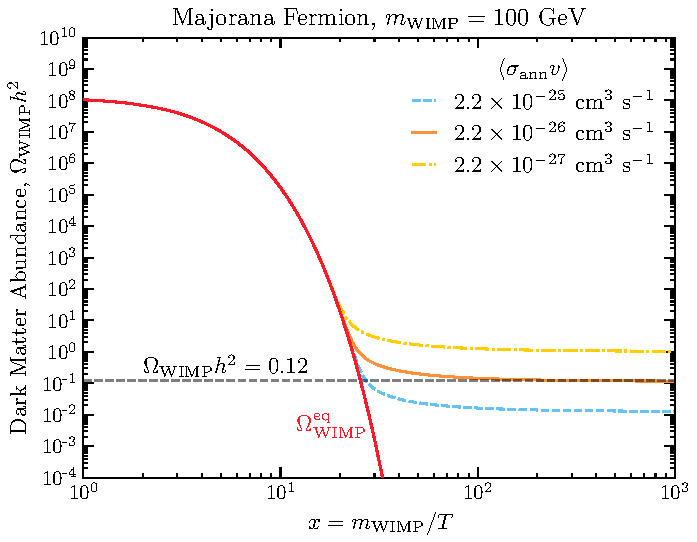
\includegraphics{fig_dm_freezeout.pdf}
    \caption[Evolution of the DM abundance as a function of $x = m_\mathrm{DM}/T$.]{Evolution of the DM abundance as a function of $x = m_\mathrm{DM}/T$. The red line tracks the abundance of the WIMP if it remains in equilibrium with the bath. The relic abundance for three different annihilation cross-sections is shown in blue, orange, and yellow for $\langle \sigma_\mathrm{ann} v\rangle = 2.2\times10^{-25},\;2.2\times10^{-26},$ and $2.2\times10^{-27}$ cm$^{3}$s$^{-1}$ respectively.}
    \label{ch1:fig:WIMP_freezeout}
\end{figure}

The allowed mass range for a thermal WIMP is between $10\MeV\lesssim m_\mathrm{WIMP} \lesssim 100\TeV$. Lighter WIMPs will make non-negligible contributions to the effective number of neutrinos at the time of Big Bang Nucleosynthesis, measured to be $N^\mathrm{BBN}_\mathrm{eff} = 3.044$~\cite{Yeh:2022heq_oct_Probingphysicsstandard}, altering the observed abundances of the light elements. The CMB offers an additional probe of $N_\mathrm{eff}$ at the later time of recombination and can be combined with the BBN result leading to the value $N_\mathrm{eff} = 2.99 \pm 0.17$~\cite{Planck:2018vyg_sep_Planck2018results}. Given the Standard Model predicts a value of $N_\mathrm{eff} = 3.044$, contributions from additional relativistic degrees of freedom must be less than $\Delta N_\mathrm{eff} < 0.28$~\cite{Yeh:2022heq_oct_Probingphysicsstandard}.  
At the high end of this range, dark matter with a mass larger than $\sim 100\TeV$ requires an annihilation cross-section larger than that permitted by partial wave unitarity of the $s$-matrix to achieve the correct relic abundance~\cite{Griest:1989wd_UnitarityLimitsMass}.  
 

\subsubsection{Axions}
The axion originally arose from the Pecci-Quinn solution to the strong CP problem. This refers to the absence of observed CP-violation in the QCD sector of the Standard Model. In principle, the SM Lagrangian should include the term
\begin{equation}
    \mathcal{L}_{\theta_\mathrm{QCD}} = \frac{g_s^2}{32 \pi}\theta_\mathrm{QCD} G_{\mu\nu} \tilde{G}^{\mu\nu},
\end{equation}
where $g_s$ is the QCD coupling constant, $G_{\mu\nu}$ is the gluon field strength tensor and $\tilde{G}^{\mu\nu}$ is its dual. This term generates an electric dipole moment for the neutron (nEDM) that has yet to be observed experimentally. The current upper bound on the nEDM is $|d_n| < 0.18\times 10^{-26}\;e\cm$~\cite{Abel:2020pzs_feb_MeasurementPermanentElectric} and can be translated to an upper bound on the CP-violating QCD $\theta$-parameter such that $|\theta_{QCD}|\lesssim 10^{-10}$, raising questions as to why this value is so small. 

The Peccei-Quinn solution to this problem introduces a new, anomalous, global  $U(1)_{\mathrm{PQ}}$ symmetry and promotes $\theta_\mathrm{QCD}$ to be a dynamical field.
Wilczek~\cite{Wilczek:1977pj_ProblemStrongInvariance} and Weinberg~\cite{Weinberg:1977ma_NewLightBoson} showed that the axion emerges as the pseudo-Goldstone boson associated with the breaking of $U(1)_\mathrm{PQ}$. Though the original axion was quickly ruled out, many modern extensions of the SM predict the existence of a QCD axion. Two of the most prominent UV completions of the axion are the KSVZ~\cite{Kim:1979if_WeakInteractionSinglet, Shifman:1979if_CanConfinementEnsure} and DFSZ~\cite{Zhitnitsky_PossibleSuppressionAxion, Dine:1981rt_SimpleSolutionStrong} models. In these models, the axion produced in the early Universe can serve the role of cold dark matter. This makes it a very compelling dark matter candidate, as it solves two of the biggest mysteries of physics in one neat package. 

However, solving the Strong CP problem can be rather restrictive on the model parameters. For example, the QCD axion's coupling to the photon, $g_{a\gamma\gamma}$, is not a free parameter and depends on the scale at which the PQ symmetry is broken. Many models introduce a light pseudoscalar particle, say $a$, that couples to the photon in the same way as the QCD axion,  
\begin{equation}
    \mathcal{L}_{a\gamma\gamma} = -\frac{g_{a\gamma\gamma}}{4} a F_{\mu\nu}\tilde{F}^{\mu\nu},
\end{equation}
but is not associated with a solution to the Strong CP problem. Such pseudoscalars are known as ``Axion Like Particles" (ALPs) and can make a good dark matter candidate.

\subsubsection*{Primordial Black Holes}

Primordial black holes (PBHs) are formed during the early Universe through various mechanisms. The simplest mechanism predicts that PBHs are produced from the gravitational collapse of density fluctuations seeded during inflation~\cite{Hawking:1971ei_apr_Gravitationallycollapsedobjects, Carr:1974nx_Blackholesearly,Carr:1975qj_Primordialblackhole}. 
Unlike black holes that originate from stellar collapse, which have masses $\gtrsim 3\Msun$, the mass of a PBH can be arbitrary.  PBHs can also make a good dark matter candidate, satisfying all the criteria points outlined above. In fact, PBHs with a mass between $\sim (10^{-17} - 10^{-12})\;\Msun$, dubbed ``asteroid mass PBHs'', can account for 100\% of the dark matter content in the Universe~\cite{Montero-Camacho:2019jte_aug_Revisitingconstraintsasteroidmass}. Outside this range, PBHs can still make up a small fraction of dark matter~\cite{Villanueva-Domingo:2021spv_may_Briefreviewprimordial}. 

%%%%%%%%%%%%%%%%%%%%%%%%%%%%%%%%%%%%%
%%%%%%%%%%%%%%%%%%%%%%%%%%%%%%%%%%%%%
\section{Dark Matter in an Effective Field Theory Framework}
\label{ch1:subsec:DM_EFTs}
%%%%%%%%%%%%%%%%%%%%%%%%%%%%%%%%%%%%%
%%%%%%%%%%%%%%%%%%%%%%%%%%%%%%%%%%%%%

For a dark matter candidate to be truly compelling, it should be able to be embedded into an ultraviolet (UV) complete theory. Such theories are renormalisable\footnote{In a renormalisable theory, the infinities that arise from UV divergences can be absorbed by fixing a finite number of parameters to experimentally observed values.} and gauge invariant under the SM gauge group $SU(3)_\mathrm{colour}\otimes SU(2)_L\otimes U(1)_Y$. This allows these models to be predictive up to arbitrarily high energies. These theories are typically quite complex, requiring the introduction of multiple new fields and many more free parameters. As an example, consider the phenomenological Minimal Supersymmetric Standard Model (pMSSM)~\cite{Villanueva-Domingo:2021spv_may_Briefreviewprimordial} in which the lightest neutralino\footnote{The neutralinos are the mass eigenstates of the supersymmetric partners of the neutral gauge bosons and the higgsino.} can be a thermal WIMP dark matter candidate. In this theory, 19 free parameters are introduced on top of the free parameters in the SM, requiring 38 independent experimental observations to fully constrain the model. Given that, at this time, all good dark matter candidates are equally likely to be the correct one, a model-independent approach to interpreting experimental results is desirable. This is achieved by describing the interactions of dark matter with the SM through an effective field theory (EFT).

%%%%%%%%%%%%%%%%%%%%%%%%%%%%%%%%%%%%%
\subsection{Overview of Effective Field Theory}
\label{ch1:subsec:EFT_intro}
%%%%%%%%%%%%%%%%%%%%%%%%%%%%%%%%%%%%%

Modern physics can be thought of as a ladder of theories that are designed to describe the important physics present at a given energy (or length) scale. For example, Newtonian mechanics is a sufficient description of the physics experienced in our everyday lives. However, in situations where the energy is comparable to the mass of the system, Newtonian mechanics breaks down, and Special Relativity must be used to describe the physics at these energies. In particle physics, the Standard Model provides an excellent description of particle interactions up to the energies reached at LHC and perhaps even further beyond. However, even it is expected to break down at higher energy scales, in particular at the Planck scale, where a quantum theory of gravity is required. Hence, both Newtonian mechanics and the SM are low-energy, effective descriptions of a more complete theory.

This philosophy based on only describing the physics relevant below some energy scale, $\Lambda$, is the core principle of EFTs. The Lagrangian for the effective theory only contains the degrees of freedom that can be produced below the scale $\Lambda$, i.e. fields that have masses less than this scale. This low-energy regime described by the EFT is often called the infrared (IR) regime. 

In general, the EFT Lagrangian will contain renormalizable terms, $\mathcal{L}_\mathrm{renorm.}$,  built out of operators that have mass dimension $\leq 4$, as well as operators with mass dimension $n> 4$, denoted $\mathcal{O}_i^{(n)}$, that encapsulate the contributions from the UV physics. Each of these higher dimensional operators will be suppressed by the scale of new physics, $\Lambda^{4-n}$. 
The effective Lagrangian can then be written as
\begin{equation}
    \mathcal{L}_\mathrm{EFT} = \mathcal{L}_\mathrm{renorm.} +  \sum_{n>4}   \sum_{i = 1}^{j_n} \frac{C_i^{(n)} (\tilde{\mu})}{\Lambda^{n-4}}\mathcal{O}_i^{(n)},
    \label{ch1:eq:EFT_Lagrangian}
\end{equation}
where we sum over all $j_n$ operators present at mass dimension $n$. The expansion coefficients, $C_i^{(n)}$, are the Wilson coefficients that depend on the details of the UV physics. In general, the Wilson coefficients run with the energy scale, $\tilde{\mu}$, with this evolution described by the renormalisation group equations (RGEs).
The sum over the mass dimension of the operators is typically terminated at some sensible value, as higher dimensional operators get increasingly suppressed by the cutoff scale $\Lambda$.

The series of operators in Eq.~\ref{ch1:eq:EFT_Lagrangian} can be constructed in two different ways. First, we assume some prior knowledge of the underlying UV theory. Then, for a given energy scale $\Lambda$, the heavy degrees of freedom are known, and can be explicitly integrated out. There are various methods for performing this process, the simplest being expanding the propagator of the heavy fields in powers of the momenta over the heavy mass, $(p/M)^2$. For the simple case of a heavy scalar, this corresponds to 
\begin{equation}
    \frac{i}{p^2 - M^2} = \frac{-i}{M^2}\left(\frac{1}{1 - (p/M)^2}\right)\approx \frac{-i}{M^2}\left( 1 + \left(\frac{p}{M}\right)^2 + \mathcal{O}\left(\left(\frac{p}{M}\right)^4\right)\right).
\end{equation}
An alternate method is to replace the heavy fields in the Lagrangian with their classical equations of motion. The resulting effective Lagrangian will contain all the operators generated by the UV theory at tree level.
Constructing an EFT in this way is called the \textit{top-down} method.

The second method of constructing an EFT is to be agnostic to the UV physics and write down all possible operators that can be constructed from the IR degrees of freedom. These operators must obey the symmetries of the IR theory, as well as any other constraints one wishes to impose\footnote{For example, one might require that no flavour changing processes are present at dimension 5, despite such operator being allowed by the symmetries.}. This is the \textit{bottom-up} approach, offering a more model-independent approach than the top-down method. The Wilson coefficients, in this case, will be arbitrary functions of the energy scale determined by solving the RGEs.

In general, the parameter space of the EFT will be lower dimensional than those of the corresponding UV models. This allows for an easier comparison with experimental results, as fewer parameters need to be fit to the data. Once the Wilson coefficients have been constrained at the low energy scale of the experiments, they can be matched to the coefficients generated by some UV theory at another scale, thereby constraining the UV parameters. 

\subsection{Dimension 6 EFT Operators for Dirac Fermion Dark Matter}
This work will focus on dimension 6 EFT operators that describe the interactions of Dirac fermion dark matter with standard model fermions. These operators will have a structure 
\begin{equation}
    \mathcal{L}_\mathrm{EFT}^{(6)} \sim \frac{1}{\Lambda^2}(\bar{\chi}\Gamma_\mathrm{DM} \chi)(\bar{f}\Gamma_{\mathrm{SM}}f),
\end{equation}
where the $\Gamma_i$ determines the Lorentz structure of the interaction by taking appropriate combinations from the set
\begin{equation}
    \Gamma_i\in \{1, i\gamma_5, \gamma^\mu, i\gamma^\mu \gamma^5, \sigma^{\mu\nu}, i \sigma^{\mu\nu}\gamma^5\}.\label{ch1:eq:Lorentz_structure}
\end{equation}
For example, the case of $\Gamma_\chi = \Gamma_\mathrm{SM} = 1$ yields scalar currents for both the DM and SM fermions and would correspond to integrating out a heavy scalar mediator in the UV theory. Under the assumption of minimal flavour violation (MFV)\footnote{MFV is the assumption that the only source of flavour violation in the quark sector comes from the SM Yukawa matrices and not from any new physics introduced at a higher scale.}, there are ten operators at dimension six that form a linearly independent basis. These are given in Table~\ref{ch1:tab:opers_defn_full}, along with spin-averaged squared matrix element for dark matter scattering with a fermion. 
The operators are classified based on the Lorentz structures of the two bilinears, namely; Scalar (S), Pseudoscalar (P), Vector (V), Axial-vector (A), and Tensor (T), for each respective element of Eq.~\ref{ch1:eq:Lorentz_structure}.
The coupling constant, $g_f$, for operators that involve the S and P fermion bilinears (operators D1-4) are normalised by the corresponding Yukawa couplings as prescribed by MFV to avoid large flavour-changing neutral currents. The remaining bilinears have coupling constants that depend only on the cutoff scale, $\Lambda_f$.

Note that, in general, the cutoff scale for DM couplings to quarks will be different from that for leptons. The details of how these scales are connected, if they are connected at all, depend on UV physics. As such, we will only assume coupling to either quarks or leptons at the tree level. 


\begin{table}[t!bp]
\centering
\setlength{\tabcolsep}{0.25em}   
\begin{tabular}{  c  c  c  c  c }
\toprule
  Name & Operator & $g_f$  & $|\overline{\mathcal{M}}(s,t,m_i)|^2$   \\\midrule\midrule
  D1 & $\bar\chi  \chi\;\bar f  f $ & $\frac{y_f}{\Lambda_f^2}$  & $ g_f^2\frac{\left(4 m_{\chi }^2-t\right) \left(4 m_{\chi }^2-\mu ^2   t\right)}{\mu ^2}$ \\  
  D2 & $\bar\chi \gamma^5 \chi\;\bar f f $ & $i\frac{y_f}{\Lambda_f^2}$ & $g_f^2\frac{t \left(\mu ^2 t-4 m_{\chi }^2\right)}{\mu ^2}$ \\  
  D3 & $\bar\chi \chi\;\bar f \gamma^5  f $&  $i\frac{y_f}{\Lambda_f^2}$  &  $g_f^2 t \left(t-4 m_{\chi }^2\right)$ \\ 
  D4 & $\bar\chi \gamma^5 \chi\; \bar f \gamma^5 f $ & $\frac{y_f}{\Lambda_f^2}$  & $g_f^2 t^2$  \\
  D5 & $\bar \chi \gamma_\mu \chi\; \bar f \gamma^\mu f$ & $\frac{1}{\Lambda_f^2}$ &  $2 g_f^2 \frac{2 \left(\mu ^2+1\right)^2 m_{\chi }^4-4 \left(\mu ^2+1\right) \mu ^2 s m_{\chi }^2+\mu ^4 \left(2 s^2+2 s t+t^2\right)}{\mu^4}$ \\ 
  D6 & $\bar\chi \gamma_\mu \gamma^5 \chi\; \bar  f \gamma^\mu f $ & $\frac{1}{\Lambda_f^2}$ & $2  g_f^2\frac{2 \left(\mu ^2-1\right)^2 m_{\chi }^4-4 \mu ^2 m_{\chi }^2 \left(\mu ^2 s+s+\mu ^2 t\right)+\mu ^4 \left(2 s^2+2 s   t+t^2\right)}{\mu^4}$ \\ 
  D7 & $\bar \chi \gamma_\mu  \chi\; \bar f \gamma^\mu\gamma^5  f$ & $\frac{1}{\Lambda_f^2}$ &  $2  g_f^2 \frac{2 \left(\mu ^2-1\right)^2 m_{\chi }^4-4 \mu ^2 m_{\chi }^2 \left(\mu ^2 s+s+t\right)+\mu ^4 \left(2 s^2+2 s t+t^2\right)}{\mu^4}$ \\  \
  D8 & $\bar \chi \gamma_\mu \gamma^5 \chi\; \bar f \gamma^\mu \gamma^5 f $ & $\frac{1}{\Lambda_f^2}$ & $2  g_f^2 \frac{2 \left(\mu ^4+10 \mu ^2+1\right) m_{\chi }^4-4 \left(\mu ^2+1\right) \mu ^2  m_{\chi }^2 (s+t)+\mu ^4 \left(2 s^2+2 s t+t^2\right)}{\mu ^4}$ \\  
  D9 & $\bar \chi \sigma_{\mu\nu} \chi\; \bar f \sigma^{\mu\nu} f $ & $\frac{1}{\Lambda_f^2}$ & $8  g_f^2 \frac{4 \left(\mu ^4+4 \mu ^2+1\right) m_{\chi }^4-2 \left(\mu ^2+1\right) \mu ^2 m_{\chi  }^2 (4 s+t)+\mu ^4 (2 s+t)^2}{\mu ^4}$ \\  
 D10 & $\bar \chi \sigma_{\mu\nu} \gamma^5\chi\; \bar f \sigma^{\mu\nu} f $ & $\frac{i}{\Lambda_f^2}$ &  $8  g_f^2\frac{4 \left(\mu ^2-1\right)^2 m_{\chi }^4-2 \left(\mu ^2+1\right) \mu ^2 m_{\chi }^2 (4 s+t)+\mu ^4 (2 s+t)^2}{\mu^4}$\\  \bottomrule
\end{tabular}
\caption[Dimension 6 EFT operators~\cite{Goodman:2010ku_ConstraintsDarkMatter} for the coupling of Dirac DM to fermions.]{Dimension 6 EFT operators~\cite{Goodman:2010ku_ConstraintsDarkMatter} for the coupling of Dirac DM to fermions (column 2), together with the squared matrix elements DM-fermion scattering (column 5), where $s$ and $t$ are Mandelstam variables, $\mu=m_\chi/m_T$, and $m_T$ is the target mass. 
\label{ch1:tab:opers_defn_full} }
\end{table}

\subsection{From DM-Quark to DM-Nucleon Interactions}
\label{ch1:subsec:quark_to_nucleon_EFT}

The operators in Table~\ref{ch1:tab:opers_defn_full} describe dark matter interactions at the quark level, as these are the degrees of freedom most models are formulated with. However, we will primarily be interested in dark matter scattering with baryons, which requires taking the matrix element of the quark operators between baryon states, i.e. $\langle {\cal B} | \bar q \, \Gamma_q q| {\cal B}\rangle$. These matrix elements can be calculated through the application of Chiral Perturbation Theory (ChPT), giving a baryon level EFT. The operators of this EFT will have the same form as those in Table~\ref{ch1:tab:opers_defn_full}, with the obvious replacement of $f\rightarrow \cal B$, as well as additional form factors that take into account the structure of the baryons.

The required form factors for each operator have been calculated at zero momentum transfer in Ref.~\cite{Cirelli:2013ufw_oct_Toolsmodelindependentbounds} and are given by 
\begin{align}
c_{\cal B}^S(0) &= \frac{2 m_{\cal B}^2}{v^2}\left[\sum_{q=u,d,s}f_{T_q}^{(\cal B)}+\frac{2}{9}f_{T_G}^{(\cal B)}\right]^2,\label{ch1:eq:cBS}\\
c_{\cal B}^P(0) &= \frac{2 m_{\cal B}^2}{v^2}\left[\sum_{q=u,d,s}\left(1-3\frac{\overline{m}}{m_q}\right)\Delta_q^{(\cal B)}\right]^2,\label{ch1:eq:cBP}\\
c_{\cal B}^V(0) &= 9,\label{ch1:eq:cBV}\\
c_{\cal B}^A(0) &=  \left[\sum_{q=u,d,s}\Delta_q^{(\cal B)}\right]^2,\label{ch1:eq:cBA}\\
c_{\cal B}^T(0) &= \left[\sum_{q=u,d,s}\delta_q^{(\cal B)}\right]^2,\label{ch1:eq:cBT}
\end{align}
where  $v=246$ GeV is the vacuum expectation value of the SM Higgs field, $\cal B$ is the baryonic species,  $\overline{m}\equiv(1/m_u+1/m_d+1/m_s)^{-1}$ and $f_{T_q}^{(\cal B)}$, $f_{T_G}^{(\cal B)}=1-\sum_{q=u,d,s} f_{T_q}^{(\cal B)}$, $\Delta_q^{(\cal B)}$ and $\delta_q^{(\cal B)}$ are the hadronic matrix elements, determined either experimentally or by lattice QCD simulations. The specific values of these matrix elements for various baryons are provided in Appendix~\ref{appendix:hadronic_matrix_elements}.

The assumption of zero-momentum transfer is valid when considering interactions with momentum transfers $\lesssim 1\GeV$, such as in direct detection experiments. Once the momentum transfer exceeds this, the internal structure of the baryon begins to be resolved, and an additional momentum-dependent form factor is required to account for this~\cite{Thomas_ElectromagneticStructureNucleon},
\begin{equation}
    F_{\cal B}(t) = \frac{1}{\left( 1 - t/Q_0^2\right)^2},
\end{equation}
where $t$ is the Mandelstam variable, and $Q_0$ is an energy scale that depends on the hadronic form factor. For simplicity, we will conservatively take $Q_0 = 1 \GeV$ for all operators. We base this on the known values of the hadronic matrix elements~\cite{Zanotti:2017bte_Transversespindensities,Alarcon:2017ivh_Nucleonformfactors} that show values of $Q_0$ between $0.9\pm 0.1\GeV$ hold for all operators in Table~\ref{ch1:tab:opers_defn_full}.
Putting everything together, the squared coupling constants for dark matter-baryon interactions are obtained by making the replacement
\begin{equation}
    g_f^2 \rightarrow \frac{c^I_{\cal B}(t)}{\Lambda_q^4} \equiv \frac{1}{\Lambda_q^4}c_{\cal B}^I(0)F^2_{\cal B}(t),\quad I\in {S, P, V, A, T},
\end{equation}
in the matrix elements in the final column of Table~\ref{ch1:tab:opers_defn_full}.



%%%%%%%%%%%%%%%%%%%%%%%%%%%%%%%%%%%%%
%%%%%%%%%%%%%%%%%%%%%%%%%%%%%%%%%%%%%
%%%%%%%%%%%%%%%%%%%%%%%%%%%%%%%%%%%%%
\section{Current Status of Dark Matter Constraints}
%%%%%%%%%%%%%%%%%%%%%%%%%%%%%%%%%%%%%
%%%%%%%%%%%%%%%%%%%%%%%%%%%%%%%%%%%%%
%%%%%%%%%%%%%%%%%%%%%%%%%%%%%%%%%%%%%

In this section, we review the current status of dark matter detection searches, focusing on WIMP-like dark matter 
The detection methods employed to search for WIMP-like dark matter can be broadly broken down into categories that are often termed ``make it, shake it, or break it". ``Make it" refers to the production of dark matter at colliders; ``break it" to dark matter annihilation signals; and ``shake it" to dark matter scattering. 


%%%%%%%%%%%%%%%%%%%%%%%%%%%%%%%%%%%%%
%%%%%%%%%%%%%%%%%%%%%%%%%%%%%%%%%%%%%
\subsection{Collider Bounds}
%%%%%%%%%%%%%%%%%%%%%%%%%%%%%%%%%%%%%
%%%%%%%%%%%%%%%%%%%%%%%%%%%%%%%%%%%%%

If dark matter is produced in a collider, it will simply leave the detector without depositing any energy. To determine if such an invisible particle was produced, conservation of energy-momentum is used to determine if any events are missing energy. In practice, what is searched for is missing momentum that is transverse to the beamline.
The ATLAS and CMS experiments at the LHC have performed analyses on various dark matter production mechanisms, including the exchange of a $Z/Z'$ or Higgs, EFTs and heavy mediators, and mono-jet searches~\cite{CMS:2017jdm_jul_Searchdarkmatter}\footnote{These searches refer to a single jet being produced alongside a pair of dark matter particles. This jet could be of Standard Model or dark sector origin, with the latter commonly referred to as ``mono-X" searches.}. 

Currently, dark matter has not been observed to be produced in particle colliders. This non-observation has instead been used to constrain the dark matter mass and production cross-sections or couplings of various models. 
These limits are typically interpreted in a model-dependent manner, as different dark matter - Standard model couplings can significantly alter the production rates. Collider searches also offer complimentary probes of the dark matter-nucleon scattering cross-Section~\cite{Ruppin:2014bra_oct_Complementaritydarkmatter} as they probe the same underlying coupling of dark matter to quarks.  
% As mentioned above, EFTs can be used to explore a variety of interactions in a somewhat model-independent way.
% However, many applications of this nature did not hold up to scrutiny, as the EFTs were being applied at energies outside their regions of validity~\cite{Busoni:2013lha_jan_ValidityEffectiveField, Buchmueller:2013dya_EffectiveFieldTheory, Busoni:2014haa_ValidityEffectiveField, Busoni:2014sya_ValidityEffectiveField}, and so care is needed when applying such methods. 

 
 It is important to note that an observation of an invisible massive particle at a collider is not enough to infer that it is dark matter. Such an observation will only tell us that such a particle exists. On its own, it does not determine the abundance of the species or if it is stable on cosmological times. As such, it could be just a component of a larger dark sector. To measure enough of the model parameters and determine these important properties, complementary information from direct or indirect detection is often required. 
 
%%%%%%%%%%%%%%%%%%%%%%%%%%%%%%%%%%%%%
%%%%%%%%%%%%%%%%%%%%%%%%%%%%%%%%%%%%%
\subsection{Direct Detection Searches}
\label{ch1:subsec:DDsearches}
%%%%%%%%%%%%%%%%%%%%%%%%%%%%%%%%%%%%%
%%%%%%%%%%%%%%%%%%%%%%%%%%%%%%%%%%%%%
The techniques employed in direct detection experiments depend on the dark matter mass range they are attempting to probe.
For ALP dark matter that is wavelike, haloscope experiments 
such as ADMX~\cite{ADMX:2009iij_SQUIDbasedmicrowavecavity} and MADMAX~\cite{MADMAX:2019pub_mar_Newexperimentalapproach} 
attempt to convert ALPs to photons via the Primakoff effect. 
Searches for WIMP-like dark matter look for the dark matter scattering with some detector
material, causing it to recoil and deposit energy into the detector. Given that our focus is on WIMP-like dark matter, 
this section will review the status of these experiments.

The differential rate at which the incoming flux of dark matter particles will scatter within a detector containing $N_T$ targets, as a function of the recoil energy, $E_R$, is given by
\begin{equation}
    \frac{d R(E_R, t)}{dE_R} = N_T \frac{\rho_\mathrm{DM}}{m_\mathrm{DM}}\int_{v>v_\mathrm{min}}^{v_\mathrm{esc}}v f(\vec{v} + \vec{v}_E)\frac{d\sigma}{dE_R}\,d^3v,
    \label{ch1:eq:DD_rate}
\end{equation}
 where the quantities in this expression are:
\begin{itemize}
    % \item $\rho_\mathrm{DM}$ is the ambient dark matter density;
    % \item $m_\mathrm{DM}$ is the dark matter mass;
    \item the minimum dark matter velocity required by kinematics for a scattering event to occur $v_\mathrm{min}$,
    \item the Milky Way escape velocity $v_\mathrm{esc} = 528\km\s^{-1}$,
    \item the velocity of the Earth through the dark matter halo\footnote{This accounts for the orbit of the Earth around the Sun, which induces an annual modulation in the flux of DM.}, $\vec{v}_E$,
    \item the dark matter velocity distribution in the Earth's frame, $f(\vec{v} - \vec{v}_E)$, 
    \item and the differential scattering cross-section, $d\sigma/dE_R$.
\end{itemize}
The expected event rate is expected to be very low, below $\sim 1$ event per day, per kilogram of target material, per kiloelectronvolt deposited. To observe such a low event rate, these experiments must be placed in extremely low background environments. In most cases, detectors that search for dark matter scattering are placed deep underground, in laboratories that are naturally shielded from the majority of the cosmic rays incident on the surface. 

The particle physics input into the scattering rate is encapsulated within the differential cross-section, $d\sigma/dE_R$. It is common to separate the cross-section into contributions from spin-dependent (SD) and spin-independent (SI) interactions such that
\begin{align}
    \frac{d\sigma}{dE_R} & = \frac{(\mdm + m_\mathrm{T})^2}{ m_T \mdm^2 v^2}\left(\sigma^\mathrm{SI}|F_\mathrm{SI}(E_R)|^2 + \sigma^\mathrm{SD}|F_\mathrm{SD}(E_R)|^2\right),\\
    \sigma^\mathrm{SI} & \approx   \sigma^\mathrm{SI}_{0}A_T^2\left(\frac{m_T}{m_p}\right)^2 \left( \frac{m_\mathrm{DM} + m_p}{\mdm + m_T}\right)^2,\\
    \sigma^\mathrm{SD} & \approx \sigma^\mathrm{SD}_{0}\left( \frac{4(J_T + 1)}{3 J_T}\left| \langle S_p\rangle + \langle S_n\rangle \right|^2 \right) \left(\frac{m_T}{m_p}\right)^2 \left( \frac{m_\mathrm{DM} + m_p}{\mdm + m_T}\right)^2,
\end{align}
where $m_T$, $A_T$, $J_T$ are the target mass, atomic mass number, and atomic spin, $m_p$ is the mass of the proton, $\langle S_{p,n}\rangle$ are the expectation values of the protons and neutrons in the nucleus. The $\sigma^{\mathrm{SI/SD}}_{p,0}$ are reference DM-proton scattering cross-sections evaluated in the zero-momentum transfer limit, with the form factors $F_{\mathrm{SI/SD}}(E_R)$ depending on the recoil energy accounting for the finite size of the nucleus being probed at high momentum transfer.
We have assumed that dark matter interacts the same with neutrons and protons for simplicity. 

As SI interactions couple to all the nucleons in the nucleus equally, the total dark matter-nucleus cross-section is a coherent sum over all the nucleons. This results in an $A_T^2$ enhancement compared to the dark matter-nucleon cross-section. Experiments searching for SI interactions take advantage of this by using heavy noble gases as the target material, such as Xenon and Argon. On the other hand, the SD interactions do not benefit from this coherent enhancement. As the total cross-section is the sum of all the nucleon contributions, the result is expected to average out to zero unless there is an unpaired nucleon present. Materials that contain $\ce{^{19}F}$, such as perfluorobutane $C_4F_{10}$, are the favourable targets as they contain an unpaired proton.


\begin{figure}
    \centering
    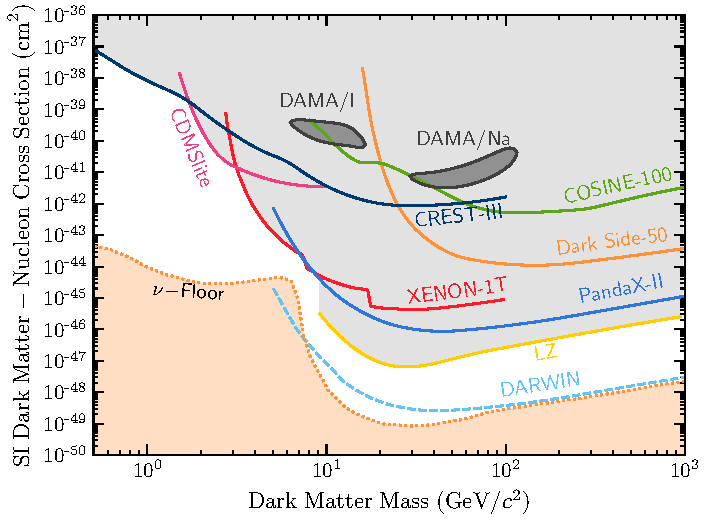
\includegraphics{DM_limits_SI.pdf}
    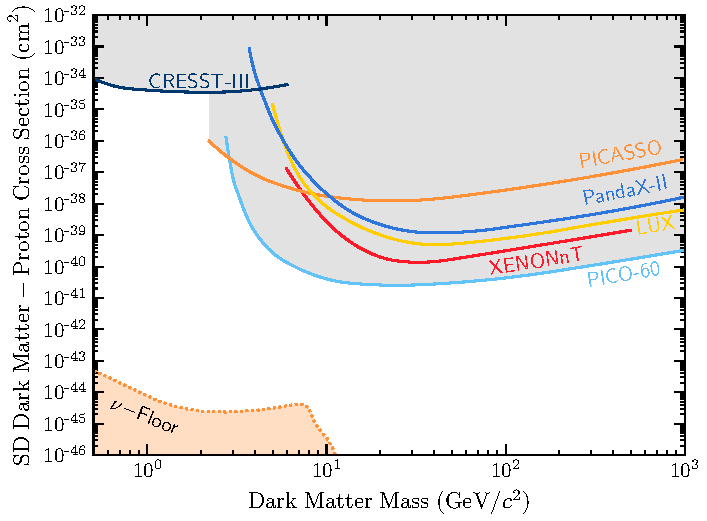
\includegraphics{DM_limits_SD_p.pdf}
    \caption[Current status of direct detection searches for dark matter.]{Current status of direct detection searches for dark matter. \textbf{Top:} Spin-independent dark matter-nucleon scattering. \textbf{Bottom:} Spin-dependent dark matter-proton scattering. Shaded regions above the coloured lines are excluded. Data was taken from the sources cited in the text.}
    \label{ch1:fig:direct_detection_lims}
\end{figure}

The current leading constraints on the dark matter-nucleon scattering cross-section
are shown in Fig.~\ref{ch1:fig:direct_detection_lims}, with SI in the top panel and SD in the bottom.
The SI limits are set by liquid noble gas experiments (LZ~\cite{LZ:2022lsv_jul_FirstDarkMatter}, 
XENON-1T~\cite{XENON:2020gfr_mar_SearchCoherentElastic}, PandaX-II~\cite{PandaX-4T:2021bab_dec_DarkMatterSearch},
and DarkSide-50~\cite{DarkSide:2022dhx_mar_SearchDarkMatterNucleon}), solid-state cryogenic detectors (CRESST-III~\cite{CRESST:2019jnq_nov_FirstresultsCRESSTIII}, CDMSlite~\cite{SuperCDMS:2023sql_jun_SearchLowmassDark}, with projected DARWIN sensitivities~\cite{Aalbers:2022dzr_dec_Nextgenerationliquidxenon}), 
and room temperature crystals (DAMA/LIBRA~\cite{Savage:2008er_CompatibilityDAMALIBRA}, and COSINE-100~\cite{COSINE-100:2021xqn_nov_StrongconstraintsCOSINE100}). 

The constraints on the SD dark matter-proton scattering cross-section are shown in the bottom panel of Fig~\ref{ch1:fig:direct_detection_lims}. 
Superheated liquid experiments such as the PICO-60~\cite{PICO:2019vsc_jul_Darkmattersearch} as well as PICASSO~\cite*{Behnke:2016lsk_apr_FinalResultsPICASSO} provide the leading constraints. 
These interactions are also constrained by many of the same experiments that focus on SI interactions, as they will inevitably contain isotopes with non-zero spin, such as $\ce{^{129} Xe}$ and $\ce{^{131} Xe}$ in XENONnT. 

The orange dashed line represents the neutrino floor\footnote{Calling this the ``neutrino fog" rather than floor has been gaining traction in recent years~\cite{OHare:2021utq_dec_Foghorizonnew}.}, providing a lower limit on the cross-section that can be probed by conventional direct detection experiments. Below this line, detectors will become sensitive to the irreducible background from Coherent Elastic Neutrino-Nucleus Scattering (CE$\nu$NS). For dark matter masses $\lesssim 10\GeV$, the solar neutrino flux is the main background source, while the atmospheric neutrino flux becomes the dominant background for masses $\gtrsim 20\GeV$. 
A significant amount of effort is being put toward overcoming this limitation, with the main strategy being to take advantage of the directionality of dark matter flux~\cite{Grothaus:2014hja_jun_DirectionalDarkMatter}. Such experiments attempt to resolve the direction of the nuclear recoil event, giving information about the direction the incident particle came from. This could allow discrimination between dark matter events, which are expected to peak in the direction of the Cygnus constellation, and the background solar and atmospheric neutrinos. 

Many experiments begin to lose sensitivity to low-mass dark matter ($m_\mathrm{DM}\lesssim 10\GeV$) as the recoil energy of the targets falls below the threshold energy resolution of the detector. Current detectors can reach thresholds as low as $\sim {\cal O} (100\eV)$, which is on the same order of magnitude as the recoil energy due to a $1\GeV$ dark matter collision. 

On the other hand, above $\sim 10\GeV$, the sensitivities of the experiments all decrease at a rate inversely proportional to the dark matter mass.  This is due to the interaction rate in Eq.~\ref{ch1:eq:DD_rate} being proportional to the number of dark matter particles that pass through the detector, $\NDM = \rho_\mathrm{DM}/m_\mathrm{DM}$. As the local dark matter density is observed to be $\rho_\mathrm{DM} = 0.4\GeV \cm^{-3}$, $\NDM$ decreases as the dark matter mass increases, and hence so do the detector sensitivities. 

Direct detection limits also assume that the scattering cross-section is independent of the dark matter velocity and momentum transfer in the interaction. Given that the local dark matter dispersion velocity is predicted to be $v_d = 270\km\s^{-1} \approx 10^{-3}c$, a back-of-the-envelope estimation for the momentum transfer gives $q_\mathrm{tr}\lesssim 100 \MeV$. Therefore, cross-sections proportional to $v_\mathrm{DM}$ or $q_\mathrm{tr}$ will result in significantly lower event rates and hence much weaker limits than the unsuppressed interactions. 

%%%%%%%%%%%%%%%%%%%%%%%%%%%%%%%%%%%%%
%%%%%%%%%%%%%%%%%%%%%%%%%%%%%%%%%%%%%
\subsection{Indirect Detection}
%%%%%%%%%%%%%%%%%%%%%%%%%%%%%%%%%%%%%
%%%%%%%%%%%%%%%%%%%%%%%%%%%%%%%%%%%%%

This leads us to indirect detection methods, which can provide complementary probes to direct detection while also exploring interactions that are difficult, if not impossible, for terrestrial-based detectors to observe.
Indirect detection experiments aim to infer the presence of dark matter through its annihilation or decay into Standard Model states. 
These searches look for dark matter annihilation products from astrophysical sources, including:
\begin{itemize}
    \item Gamma-rays at terrestrial-based telescopes such as HESS~\cite{HESS:2018cbt_may_SearchgRayLine, Montanari:2023bzn_jul_Searchdarkmatter, HESS:2006zwn_ObservationsGalacticCenter}, VERITAS~\cite{VERITAS:2017tif_apr_DarkMatterConstraints, Ryan:2023yzu_jul_SearchDarkMatter, McGrath:2023oto_jul_IndirectsearchDark, Ryan:2023yzu_jul_SearchDarkMatter}, MAGIC~\cite{MAGIC:2009tyk_MAGICGammaRayTelescope, MAGIC:2011nta_SearchesDarkMatter, MAGIC:2011nta_SearchesDarkMatter, MAGIC:2009tyk_MAGICGammaRayTelescope} and HAWC~\cite{HAWC:2017mfa_feb_DarkMatterLimits, HAWC:2017udy_feb_SearchDarkMatter, HAWC:2017udy_feb_SearchDarkMatter, HAWC:2017mfa_feb_DarkMatterLimits, Proper:2015xya_jul_FirstLimitsDark, Harding:2015bua_jul_DarkMatterAnnihilation} as well as the Fermi-LAT~\cite{Fermi-LAT:2015att_nov_SearchingDarkMatter,Fermi-LAT:2015kyq_jun_UpdatedSearchSpectral,Fermi-LAT:2012ugx_FermiLATSearch, Fermi-LAT:2010qeq_ConstraintsCosmologicalDark, Su:2010qj_GiantGammarayBubbles} satellite;

    \item Neutrino signals at IceCube~\cite{IceCube:2016dgk_mar_Searchannihilatingdark, IceCube:2012ugg_mar_Searchdarkmatter}, ANTARES~\cite{ANTARES:2016bxz_jun_SearchDarkMatter,ANTARES:2016obx_may_SearchSecludedDark,ANTARES:2016xuh_aug_LimitsDarkMatter}, Super-K~\cite{Super-Kamiokande:2015xms_apr_Searchneutrinosannihilation,Super-Kamiokande:2004pou_Searchdarkmatter,Feng:2008qn_TestingDarkMatter}, and will be searched for at the upcoming Hyper-K~\cite{Bell:2020rkw_sep_SearchingSubGeVDark,Bell:2021esh_nov_Searchingdarkmatter,Bell:2022ycf_nov_Darkmatterpollution}, JUNO~\cite{Franarin:2018gfk_jun_JUNOSensitivityResonant} experiments.

    \item Cosmic-Ray antimatter excess observed by the AMS-02 experiment~\cite{Giesen:2015ufa_sep_AMS02antiprotonslast, Bergstrom:2013jra_oct_NewLimitsDark}
\end{itemize}

Signals from dark matter annihilation are best searched for by looking at regions where the dark matter density is expected to be high, boosting the annihilation rate. 
Natural places to look include the Galactic Centre~\cite{Ipek:2014gua_sep_RenormalizableModelGalactic, Fermi-LAT:2017opo_may_FermiGalacticCenter}, dwarf-spheroidal galaxies~\cite{Bonnivard:2015xpq_oct_Darkmatterannihilation}, and celestial bodies where dark matter can accumulate over time. The latter scenario is directly related to the topic of this thesis and was pioneered by considering the effects of dark matter being captured within the Sun.



%%%%%%%%%%%%%%%%%%%%%%%%%%%%%%%%%%%%%
%%%%%%%%%%%%%%%%%%%%%%%%%%%%%%%%%%%%%
\section{Dark Matter Signals from the Sun}
\label{ch1:sec:solar_signals}
%%%%%%%%%%%%%%%%%%%%%%%%%%%%%%%%%%%%%
%%%%%%%%%%%%%%%%%%%%%%%%%%%%%%%%%%%%%

Stars have a rich history of being used as astrophysical laboratories to search for dark matter. Depending on the type of dark matter being searched for, various signals can be looked for.
For example, light bosonic dark matter, such as ALPs and dark photons, can be produced in the plasma of stars, altering their energy transport properties.
This can ultimately lead to deviations in the evolution of the star, which can be used to place some of the strongest constraints on these models~\cite{An:2013yfc_oct_Newstellarconstraints, Dolan:2022kul_oct_Advancingglobularcluster, Dolan:2023cjs_jun_ConstrainingDarkPhotons}.
WIMP-like dark matter particles in the halo that couples to visible matter can scatter in stars as they pass through. 
If the dark matter loses enough energy in these interactions, it can become gravitationally bound to the object and a population of dark matter will accumulate within the star over time~\cite{Press:1985ug_Capturesungalactic, Gould:1987ju_WeaklyInteractingMassive, Gould:1987ir_ResonantEnhancementsWIMP, Jungman:1995df_Supersymmetricdarkmatter, Busoni:2017mhe_oct_Evaporationscatteringmomentum}. 

This idea of WIMPs accumulating within the cores of stars has been applied extensively to the star closest to us, the Sun. The formalism for stellar capture of dark matter was set up by Gould~\cite{Gould:1987ir_ResonantEnhancementsWIMP, Gould:1987ju_WeaklyInteractingMassive,Gould:1991va_Bigbangarcheology} in the late 80's, and still forms the framework used in present-day calculations, with many authors continuing to build upon these foundations over time~\cite{Busoni:2017mhe_oct_Evaporationscatteringmomentum,Garani:2017jcj_may_DarkmatterSun,Bramante:2017xlb_sep_Multiscatterstellarcapture}.

Once the dark matter is captured, it will continue to scatter with the stellar constituents until it thermalises within the core of the Sun, collecting with an isothermal sphere. The radius of this sphere can be found by applying the virial theorem, with the gravitational potential given by
\begin{align}
    \Phi(r) & = -\int_r^\infty \,\frac{G M_\odot(r')}{r'^2}dt'\\
    &\approx \frac{2}{3}\pi G \rho_{\odot,c} r^2,
\end{align}
assuming the density of the Sun within this region is constant, $\rho_{\odot,c}$, with $M_\odot(r)$ is the mass of the Sun contained within a radius $r$. The resulting radius is
\begin{equation}
    r_\mathrm{iso}^2 = \frac{3 T_\odot}{2\pi G \mdm \rho_\odot},
\end{equation}
where $T_\odot$ is the core temperature of the Sun. The dark matter number density will follow a Gaussian profile, 
\begin{align}
    n_\mathrm{iso}(r) &= n_0\exp\left( - \frac{\mdm \Phi(r)}{T_\odot}\right)\\
     & = n_0 \exp(-r^2/r_\mathrm{iso}^2),
\end{align}
where $n_0$ is a normalisation constant fixed by requiring that the total number of dark matter particles is 
\begin{equation}
    \NDM = \int d^3 r\, \niso(r).
\end{equation}
In addition, the dark matter velocity will follow a Maxwell-Boltzmann distribution, 
\begin{equation}
    \fMB(v) = 4\pi\left(\frac{\mdm}{4\pi T_\odot}\right)^{3/2}v^2\exp\left[-\frac{\mdm v^2}{4 T_\odot}\right].
\end{equation}
%
The time evolution of the total number of dark matter particles within the Sun is governed by three processes. Capture acts to increase the number over time, while annihilation and evaporation will reduce this number over time. This is described by the differential equation
\begin{equation}
    \frac{d \NDM}{dt} = C  - E \NDM- A \NDM^2,
    \label{ch1:eq:DM_num_Sun}
\end{equation}
where $C$ and $E \NDM$ are the capture and evaporation rates respectively, with $A$ being related to the annihilation rate, $\GAnn$ through
\begin{align}
    \GAnn & = \frac{1}{2}\int\,dr^3 n_\mathrm{iso}^2(r) \sigmavdm\\
    & \equiv \frac{1}{2}A \NDM^2,
\end{align}
where the factor of 1/2 accounts for each annihilation removing two dark matter particles from the Sun. 

In this context, evaporation refers to the process in which dark matter can be ejected back out of the Sun by up-scattering\footnote{Up-scattering refers to the interactions in which the dark matter gains rather than loses energy. } off an energetic constituent. This becomes increasingly important for lighter dark matter masses, as less energy will be required to boost the dark matter above the local escape velocity. Below a certain mass, capture and evaporation come into equilibrium, and a net-zero amount of dark matter is contained within the Sun.
This critical mass places a lower bound on the dark matter mass that can be probed through stellar capture and is named the evaporation mass, $\mevap$. 

There are three regimes in which we are interested in solving Eq.~\ref{ch1:eq:DM_num_Sun}. The simplest case is when evaporation and annihilation are both negligible. In this case, the solution is simply, 
\begin{equation}
    \NDM(t) = C t,
\end{equation}
indicating that the dark matter will simply continue to grow over time.

Next,  assume that annihilations are negligible ($A = 0$) while capture and evaporation are present. The result is
\begin{equation}
    \NDM(t) = Ct\left(\frac{1 - e^{-E t}}{E t}\right),  
\end{equation}
where the first factor is the number of captured dark matter particles if evaporation is negligible. From this, we can estimate the evaporation mass by asking when the evaporation rate is large enough to cause a significant reduction in the number of captured dark matter particles relative to the $E=0$ case. This can be expressed formally as~\cite{Garani:2017jcj_may_DarkmatterSun}
\begin{equation}
    \frac{1}{\NDM(\mevap)}\left| \NDM(\mevap) - \frac{C(\mevap)}{E(\mevap)} \right| = \alpha,
\end{equation} 
where $\alpha$ is the fraction of evaporated dark matter, taken to be $\sim 10\%$. 

Finally, consider the case in which evaporation can be neglected, $\mdm\gtrsim \mevap$. The solution in this regime is
\begin{equation}
    \NDM(t) = \sqrt{\frac{C}{A}}\tanh(\sqrt{CA}t)\overset{t\rightarrow\infty}{\longrightarrow} \sqrt{\frac{C}{A}},
\end{equation}
which reaches an equilibrium state between capture and annihilation for times longer than the characteristic scale, $\teq = 1/\sqrt{CA}$. This state is known as capture-annihilation equilibrium.

The signals searched for depend on whether the dark matter can annihilate or not. If the dark matter does not have an antiparticle, as is the case in asymmetric dark matter scenarios~\cite{Petraki:2013wwa_Reviewasymmetricdark}, then it cannot annihilate, and we can set $A = 0$ in Eq.~\ref{ch1:eq:DM_num_Sun}. This leads to the population continuing to grow over time, with $\NDM(t) = Ct$ if evaporation is negligible. A large enough population of captured dark matter can alter the energy transport within the Sun, leading to the modifications of the solar neutrino flux or even the solar structure itself~\cite{Franarin:2018gfk_jun_JUNOSensitivityResonant, Cumberbatch:2010hh_LightWIMPsSun, Vincent:2013lua_apr_Thermalconductiondark, Vincent:2015gqa_aug_Generalisedformfactor}. 

Instead, if the dark matter can annihilate, an equilibrium will eventually be reached between the capture and annihilation rates, and the total number of dark matter particles will be constant. If the annihilation products can escape the Sun, they can be searched for by various experiments depending on the nature of the final states.
These could be neutrinos produced from the decays of other charged annihilation products~\cite{Super-Kamiokande:2011wjy_IndirectSearchWIMPs, Super-Kamiokande:2015xms_apr_Searchneutrinosannihilation, ANTARES:2016obx_may_SearchSecludedDark, ANTARES:2016xuh_aug_LimitsDarkMatter, IceCube:2016dgk_Searchannihilatingdark}, or to some other long-lived state that can escape the Sun and decay into visible states~\cite{Batell:2009zp_SolarGammaRays, Schuster:2009au_TerrestrialSolarLimits, Bell:2011sn_Enhancedneutrinosignals, Feng:2016ijc_jun_DarkSunshineDetecting, Leane:2017vag_jun_PowerfulSolarSignatures}.


\begin{figure}[!t]
    \centering
    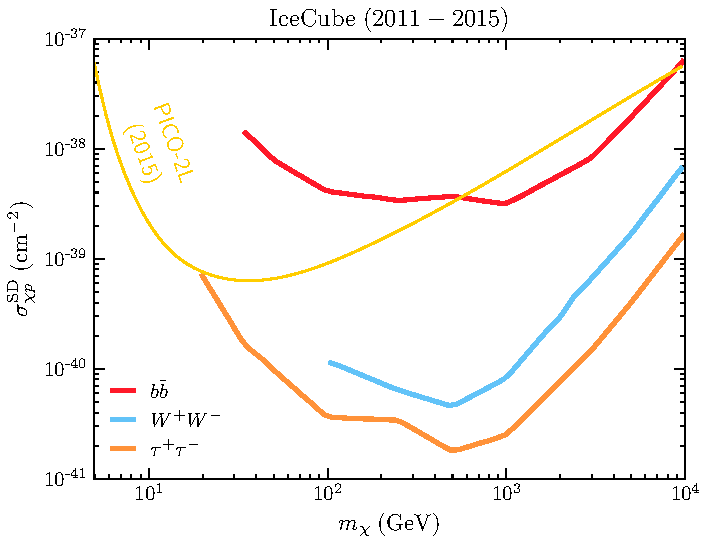
\includegraphics{IceCube_2016.pdf}
    \caption[Limits on the SD dark matter-proton cross-section from the IceCube collaboration assuming 100\% branching fraction to $b\bar{b}$ (red), $W^+ W^-$ (blue) or $\tau^+ \tau^-$ (orange) final states]{Limits on the SD dark matter-proton cross-section from the IceCube collaboration assuming 100\% branching fraction to $b\bar{b}$ (red), $W^+ W^-$ (blue) or $\tau^+ \tau^-$ (orange) final states. Also shown is the result from the PICO-2L DD experiment. This plot was recreated with data taken from Ref.~\cite{IceCube:2016dgk_mar_Searchannihilatingdark}.}
    \label{ch1:fig:IceCube_2016_SD}
\end{figure}

Interpretation of indirect detection data will require additional model-dependent assumptions, namely the relevant annihilation channels of the dark matter. The most general limits can be placed by assuming that the dark matter only has a single annihilation channel, e.g. annihilation to a $\tau^+\tau^-$ final state 100\% of the time. Under these assumptions, limits on the SD dark matter-proton cross-section have been placed that exceed current DD constraints due to the rather large abundance of Hydrogen within the Sun. Constraints from the IceCube collaboration are shown in Fig.~\ref{ch1:fig:IceCube_2016_SD}.

As stated above, the range of dark matter masses that can be probed by Solar capture is limited by the evaporation mass of $\sim 3\GeV$. Additionally, as with direct detection, interactions that are suppressed by the momentum transfer/velocity of the dark matter will result in a significantly smaller capture rate and, hence, a smaller flux of annihilation products. Ultimately, this will result in weaker constraints on the strength of dark matter interactions. These constraints also rely on the annihilation rate being sufficiently fast that capture-annihilation equilibrium is reached within the lifetime of the Sun. If the annihilation cross-section is $p$-wave suppressed by the non-relativistic velocity of the annihilating dark matter, then this equilibrium may not be achieved. Should this be the case, then no limits can be placed as the flux of annihilation products is suppressed. 

Overcoming the first of these issues requires either a colder star or one that is much heavier. Both of these scenarios will lead to a star with a lower evaporation mass, which allows probing dark matter with lighter masses. The second requires dark matter to scatter with the constituent material at relativistic energies to overcome the suppression in the cross-section. 
Finally, the annihilation rate can be enhanced if the dark matter annihilates within a smaller volume within the star. If this volume is small enough, this enhancement can compensate for the suppression that arises from $p$-wave annihilations.

Fortunately, there exist objects where all of these effects are present, allowing for a wider variety of dark matter models to be explored than direct detection or traditional indirect detection experiments. Namely, these are neutron stars and white dwarfs, stellar remnants that are extremely dense and cool to significantly lower temperatures than the centre of our Sun. These stars (along with black holes) are collectively known as compact objects, and will be the laboratories in which we study dark matter in this thesis.

%%%%%%%%%%%%%%%%%%%%%%%%%%%%%%%%%%%%%
%%%%%%%%%%%%%%%%%%%%%%%%%%%%%%%%%%%%%
%%%%%%%%%%%%%%%%%%%%%%%%%%%%%%%%%%%%%
\section{Compact Objects as Dark Matter Probes}
%%%%%%%%%%%%%%%%%%%%%%%%%%%%%%%%%%%%%
%%%%%%%%%%%%%%%%%%%%%%%%%%%%%%%%%%%%%
%%%%%%%%%%%%%%%%%%%%%%%%%%%%%%%%%%%%%

The main goal behind this work is to explore how compact objects can be used to probe a wide variety of dark matter interactions that terrestrial direct detection experiments are insensitive to. In this context, we refer to compact objects as being Neutron Stars (NSs) and White Dwarfs (WDs), and not Black Holes that often fall into this category.


Compact objects offer a unique laboratory for studying dark matter and its interactions with the Standard Model in environments unachievable anywhere else in the Universe. They generate strong gravitational fields and are composed of incredibly dense matter, with NSs reaching super-nuclear densities in their central cores. The capture rate within these objects is therefore enhanced due to these properties, with benefits over solar capture including:


\begin{itemize}
\item \textbf{Gravitational focusing of the DM flux:} The strong gravitational field will increase the impact parameter of the star. This increases the effective size of the capturing body, increasing the flux of dark matter passing through it. 

\item \textbf{Relativistic Interaction Energies:} In general, the infalling dark matter will be accelerated to (semi-)relativistic velocities ($\sim 0.2 - 0.7 c$). Moreover, the stellar constituents will also have relativistic energies. As such, interactions that are momentum/velocity dependent will suffer far less suppression than in DD experiments. 

\item \textbf{Large Number of Targets:} The extremely high densities of these objects correspond to a considerable number of scattering targets. This allows these objects to probe very small scattering cross-sections, with NSs in particular expected to reach as low as $\sim 10^ {-45}\cm^2$. 

\item \textbf{Low Evaporation Masses}: Relative to the Sun, the evaporation mass in compact objects can be quite low, on the order of keV in some cases. This is due in part to the increased gravitational strength but mainly to the significantly lower temperatures in old compact objects. 
\end{itemize}

In the past, capture in NSs has been considered primarily in the context of seeding gravitational collapse into black holes~\cite{McDermott:2011jp_ConstraintsScalarAsymmetric, Kouvaris:2011fi_ExcludingLightAsymmetric,Guver:2012ba_may_Capturedarkmatter, Garani:2018kkd_may_NewAnalysisNeutron, Bramante:2013nma_jan_Boundsselfinteractingfermion, Bertoni:2013bsa_dec_DarkMatterThermalization, Bell:2013xk_jun_Realisticneutronstar}, and the modifications of NS merger rates as well as the gravitational wave signatures produced in these events~\cite{Bramante:2017ulk_mar_SearchingDarkMatter, Ellis:2017jgp_jun_SearchDarkMatter, Ellis:2018bkr_jun_DarkMatterEffects, Nelson:2018xtr_jul_Darkhalosneutron}. Capture in WDs has also been considered, with a variety of different applications of the capture process~\cite{Steigerwald:2019efv_dec_DarkMatterThermonuclear, Panotopoulos:2020kuo_jun_Constraintslightdark, McCullough:2010ai_CaptureInelasticDark, Hooper:2010es_InelasticDarkMatter, Bramante:2015cua_sep_Darkmatterignition, Bertone:2007ae_CompactStarsDark}. 

In recent years, dark matter induced heating of NSs has reemerged as a potential detection frontier~\cite{Raj:2017wrv_feb_Neutronstarsdark, Baryakhtar:2017dbj_sep_DarkKineticHeating, Bell:2018pkk_sep_HeatingNeutronStars, Joglekar:2019vzy_sep_Relativisticcapturedark, Acevedo:2019agu_mar_WarmingNuclearPasta, Bell:2019pyc_jun_CaptureLeptophilicDark, Garani:2019fpa_aug_Darkmatterinteractions, Chatterjee:2022dhp_jul_Faintlightold}. It was shown that dark matter could reheat old, isolated NSs in our local neighbourhood\footnote{Local neighbourhood refers to the region within $\sim 1\kpc$ of the Sun.} back up to temperatures that would cause them to radiate in the near-infrared. 
For example, one might locate an NS with radio telescopes such as the Square-Kilometre-Array (SKA) and determine its age through its spin-down rate. 

Once located, the star's temperature can be determined through observations from infrared telescopes such as the James Webb Space Telescope (JWST). Knowing the age of the star allows us to compare its observed temperature to that predicted by models of neutron star cooling. A discrepancy between these two temperatures can indicate whether an additional heating source is present within the star. However, there may exist other heating mechanisms within neutron stars that could mask the effect of dark matter heating\footnote{One example of this is rotochemical heating, which has been shown to mask any potential dark matter signal~\cite{Hamaguchi:2019oev_aug_DarkMatterHeating}}. Therefore, observing an old, cold star that shows no evidence of any external heating source can provide stringent constraints on the interaction strength of dark matter with the constituents of the star. The colder the observed star, the stronger the constraints that can be placed.

This heating occurs in two stages. The dark matter will first kinetically heat the star through the scattering events that result in both its capture and thermalisation. We define \textit{kinetic hearing} to have been achieved once the dark matter has deposited $99\%$ of its initial kinetic energy into the star.
If the dark matter can annihilate, and assuming these annihilation products remain trapped within the star, its mass energy will be transferred to the star, further increasing the temperature of the star. In order for this \textit{annihilation heating} to be efficient, capture-annihilation equilibrium must be achieved on a timescale shorter than the age of the star. These processes are illustrated in Fig.~\ref{ch1:fig:cartoon_NS_heat}, with the temperatures shown assuming a NS in our local neighbourhood.


\begin{figure}[!t]
    \centering
    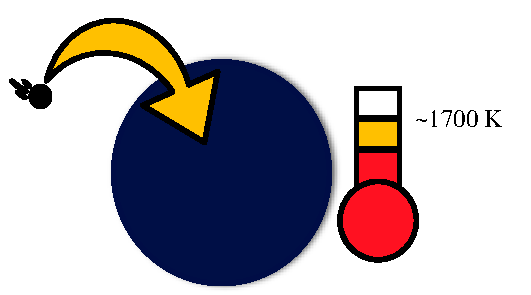
\includegraphics[width=0.45\textwidth]{kin_heat_NS.pdf}
    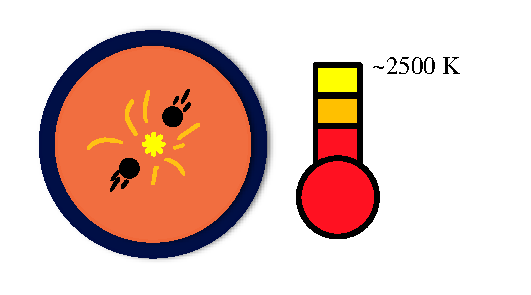
\includegraphics[width=0.45\textwidth]{ann_heat_NS.pdf}
    \caption[Illustration of DM-induced heating of compact objects.]{Illustration of DM-induced heating of compact objects. \textbf{Left:} kinetic heating due to DM scattering, raising the temperature to $\sim 1700 \K$. \textbf{Right:} Annihilation heating contributes an additional $\sim 800\K$. This image is inspired by Ref.~\cite{Raj:2017wrv_feb_Neutronstarsdark}.}
    \label{ch1:fig:cartoon_NS_heat}
\end{figure}

It is important to keep track of all the timescales involved in the heating process so that we can accurately determine the full extent of dark matter-induced heating. These timescales are the age of the star, $\tstar$, the kinetic heating time, $\tkin$, and the capture-annihilation heating timescale, $\teq$. In order for maximal heating to be achieved, we require $\tkin + \teq < \tstar$. 

To accurately project the sensitivity on the dark matter scattering cross-section that could be achieved by a future neutron star observation, one first requires an accurate calculation of the capture rate. However, existing calculations have relied on the formalism set up by Gould for capture in the Sun without fully accounting for the extreme physics present in these objects. Developing a consistent formalism for dark matter capture in compact objects, based on the Gould formalism, and applying this to dark matter induced heating is at the heart of this thesis.  

%%%%%%%%%%%%%%%%%%%%%%%%%%%%%
%%%%%%%%%%%%%%%%%%%%%%%%%%%%%
\section{Thesis Outline}
%%%%%%%%%%%%%%%%%%%%%%%%%%%%%
%%%%%%%%%%%%%%%%%%%%%%%%%%%%%

Following this introduction, Chapter~\ref{chapter:compactobjects} covers the prerequisite knowledge of compact objects
required for the remainder of this work. This includes a detailed overview of the general structure equations of relativistic stars, followed by details of the internal structure of both white dwarfs and neutron stars. 

Chapter~\ref{chapter:capture_intro} of this thesis is devoted to reformulating Gould's capture formalism to account for the physics specific to compact objects in a self-consistent manner. These include a relativistic treatment of the kinematics, using General Relativity to calculate the correct dark matter flux passing through the star, and accounting for Pauli blocking of the final state target using Fermi-Dirac statistics for the stellar constituents. In addition, we incorporate the internal structure of these objects by calculating the radial profiles for the relevant microscopic quantities (e.g., chemical potentials and number densities) via the adoption of a realistic equation of state.

The resulting formalism is sufficient to discuss dark matter scattering from leptonic species in compact objects, which are discussed in Chapter~\ref{chapter:capture_leptons}. We consider dark matter scattering with electrons and muons within neutron stars, calculating the cross-sections that may be probed by future observations. Additionally, we consider dark matter scattering with the degenerate electrons within white dwarfs. We use observations of white dwarfs in globular cluster Messier-4 to constrain the dark matter-electron scattering cross-section.

Further considerations are required when considering dark matter interactions with the baryonic matter inside NSs. Due to the high density of the NS interior, the baryons undergo strong self-interactions and should not be treated as a free Fermi gas. Instead, adopting an equation of state that accounts for these interactions is required. These interactions modify the mass of the baryons, leading them to obtain an effective mass smaller than their value in vacuum. Furthermore, as we will see, the dark matter may interact with the baryons with momentum transfers on the order of $10\GeV$. This is high enough that the dark matter will begin to resolve the internal structure of the baryon. To account for this, the momentum dependence of the baryon form factors that are typically neglected in direct detection and solar capture must be reintroduced.

This formalism is made in preparation for a thorough analysis of the timescales involved in the dark matter heating of compact objects, covered in Chapter~\ref{chapter:thermalisation}. The energy deposited in both the kinetic and annihilation heating stages does not occur instantaneously, and the timescales involved need to be compared to the age of the star in question. For annihilation heating to occur, the dark matter must first reach a state of capture-annihilation equilibrium within the stellar core. In standard calculations of this timescale, the dark matter must first become thermalised with the star. Only then can annihilations occur efficiently enough to heat the star. 


We will work with the EFT operators in Table~\ref{ch1:tab:opers_defn_full} that describe Dirac fermion dark matter interacting with Standard Model fermions. Each operator will be studied in isolation, i.e., by considering a Lagrangian that contains only one of the operators rather than a linear superposition of multiple. This way, we can analyse specific types of interactions independently, allowing us to take as model-independent an approach to the phenomenology as possible. 

We present our concluding remarks on this thesis in Chapter~\ref{chapter:conclusion}.